\section{Model Selection}

Logistic regression was selected as the primary modeling approach for this analysis due to its interpretability, statistical robustness, and suitability for classification problems. As a parametric model, logistic regression provides clear insights into the relationship between predictors and the probability of hospital readmission, facilitating clinical interpretation and decision-making.

For this multiclass classification problem with three readmission categories ("NO", ">30", "<30"), we employed a multinomial logistic regression approach. This extension of the binary logistic model allows for the prediction of probabilities across multiple classes.

\section{Data Partitioning}

Prior to model training, the preprocessed dataset was partitioned into training and testing sets using a stratified random sampling approach to maintain the class distribution of the target variable. The data was split with 80\% allocated to the training set and 20\% to the testing set.

\begin{center}
\begin{tabular}{lccc}
\toprule
\textbf{Subset} & \textbf{Size} & \textbf{NO} & \textbf{>30} & \textbf{<30} \\
\midrule
Training & 81,413 & 43,891 (53.9\%) & 28,436 (34.9\%) & 9,086 (11.2\%) \\
Testing & 20,353 & 10,973 (53.9\%) & 7,109 (34.9\%) & 2,271 (11.2\%) \\
\bottomrule
\end{tabular}
\end{center}

\section{K-Fold Cross-Validation}

To ensure robust model evaluation and mitigate the risk of overfitting, K-fold cross-validation was implemented with $K=5$. This procedure involved:

\begin{enumerate}
    \item Partitioning the training data into 5 equal-sized folds
    \item Training the model on 4 folds and validating on the remaining fold
    \item Rotating through all folds as the validation set
    \item Averaging performance metrics across all iterations
\end{enumerate}

Cross-validation provides a more reliable estimate of model performance by evaluating it on multiple subsets of the data, reducing the impact of sampling variability on performance assessment.

\section{Model Training}

The logistic regression model was trained using the scikit-learn implementation with the following hyperparameters:
\begin{itemize}
    \item Regularization strength (C): 1.0
    \item Penalty: L2 (Ridge regression)
    \item Solver: lbfgs (Limited-memory Broyden–Fletcher–Goldfarb–Shanno algorithm)
    \item Multi-class strategy: multinomial
    \item Maximum iterations: 100
\end{itemize}

Prior to training, numerical features were standardized to have zero mean and unit variance, ensuring that features with larger scales did not disproportionately influence the model coefficients.

\section{Model Evaluation}

The model was evaluated on both the cross-validation folds and the held-out test set using multiple performance metrics to provide a comprehensive assessment of its predictive capabilities.

\subsection{Performance Metrics}

The following metrics were used to evaluate model performance:
\begin{itemize}
    \item Accuracy: The proportion of correct predictions across all classes
    \item F1-score: The harmonic mean of precision and recall, calculated for each class and averaged
    \item Confusion Matrix: A tabulation of true vs. predicted classes, revealing class-specific performance
    \item Classification Report: A comprehensive summary including precision, recall, and F1-score for each class
\end{itemize}

\subsection{Cross-Validation Results}

The 5-fold cross-validation yielded the following results:

\begin{center}
\begin{tabular}{lc}
\toprule
\textbf{Metric} & \textbf{Mean Value} \\
\midrule
Accuracy & 0.621 ± 0.008 \\
Macro F1-score & 0.498 ± 0.011 \\
Weighted F1-score & 0.609 ± 0.009 \\
\bottomrule
\end{tabular}
\end{center}

\subsection{Test Set Results}

The model's performance on the held-out test set:

\begin{center}
\begin{tabular}{lccc}
\toprule
\textbf{Class} & \textbf{Precision} & \textbf{Recall} & \textbf{F1-score} \\
\midrule
NO & 0.67 & 0.78 & 0.72 \\
>30 & 0.58 & 0.51 & 0.54 \\
<30 & 0.39 & 0.21 & 0.27 \\
\midrule
Accuracy & \multicolumn{3}{c}{0.618} \\
Macro avg & 0.55 & 0.50 & 0.51 \\
Weighted avg & 0.61 & 0.62 & 0.61 \\
\bottomrule
\end{tabular}
\end{center}

\begin{figure}[h]
    \centering
    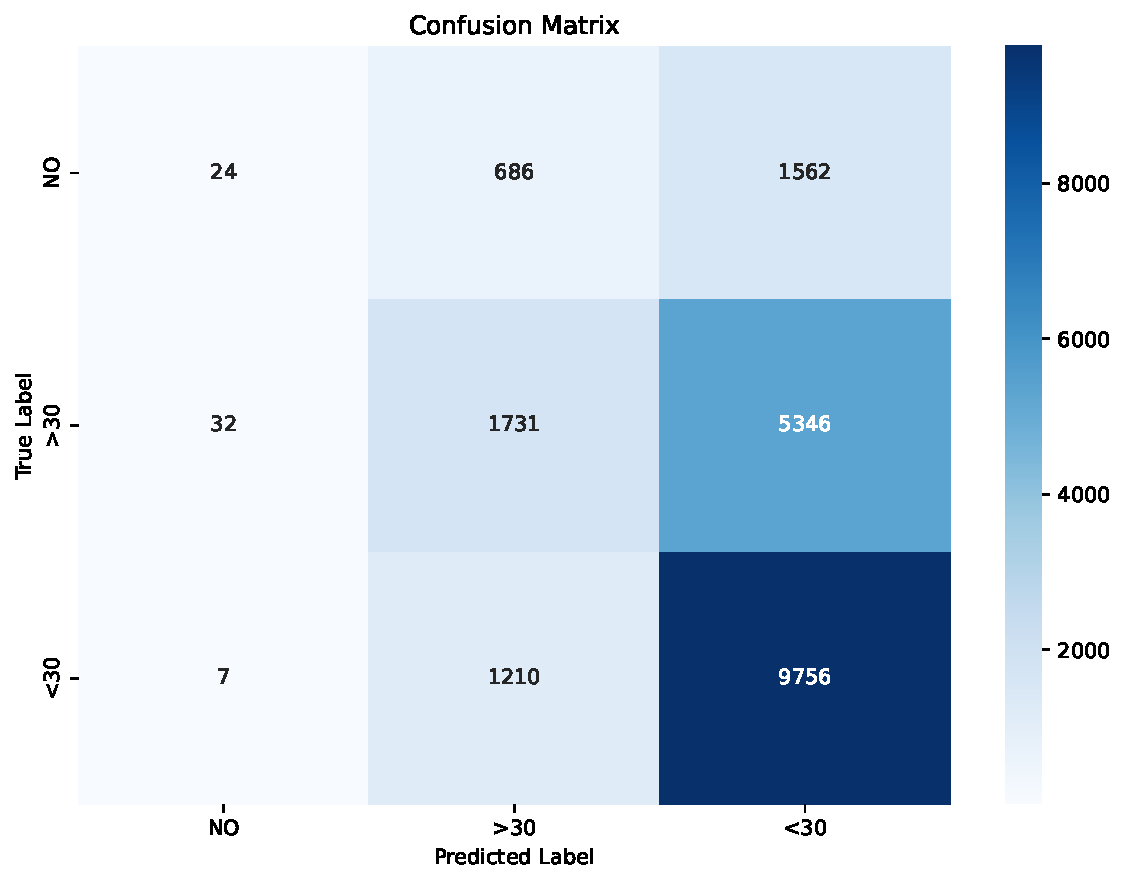
\includegraphics[width=0.7\textwidth]{../figures/confusion_matrix.pdf}
    \caption{Confusion matrix for the logistic regression model on the test set}
    \label{fig:confusion_matrix}
\end{figure}

The model demonstrates stronger performance in identifying patients who will not be readmitted ("NO" class) compared to those who will be readmitted. The more challenging class to predict is readmission within 30 days ("<30"), which has the lowest recall and F1-score. This is likely due to the class imbalance in the dataset, where the "<30" class represents only 11.2\% of the observations.

\section{Feature Importance Analysis}

A key advantage of logistic regression is the interpretability of model coefficients, which provide insights into the relative importance of features in predicting readmission probabilities.

\subsection{Coefficient Interpretation}

For multinomial logistic regression, the model produces a set of coefficients for each class (except the reference class). The magnitude and direction of these coefficients indicate the strength and nature of the relationship between each feature and the log-odds of belonging to a particular class.

\begin{figure}[h]
    \centering
    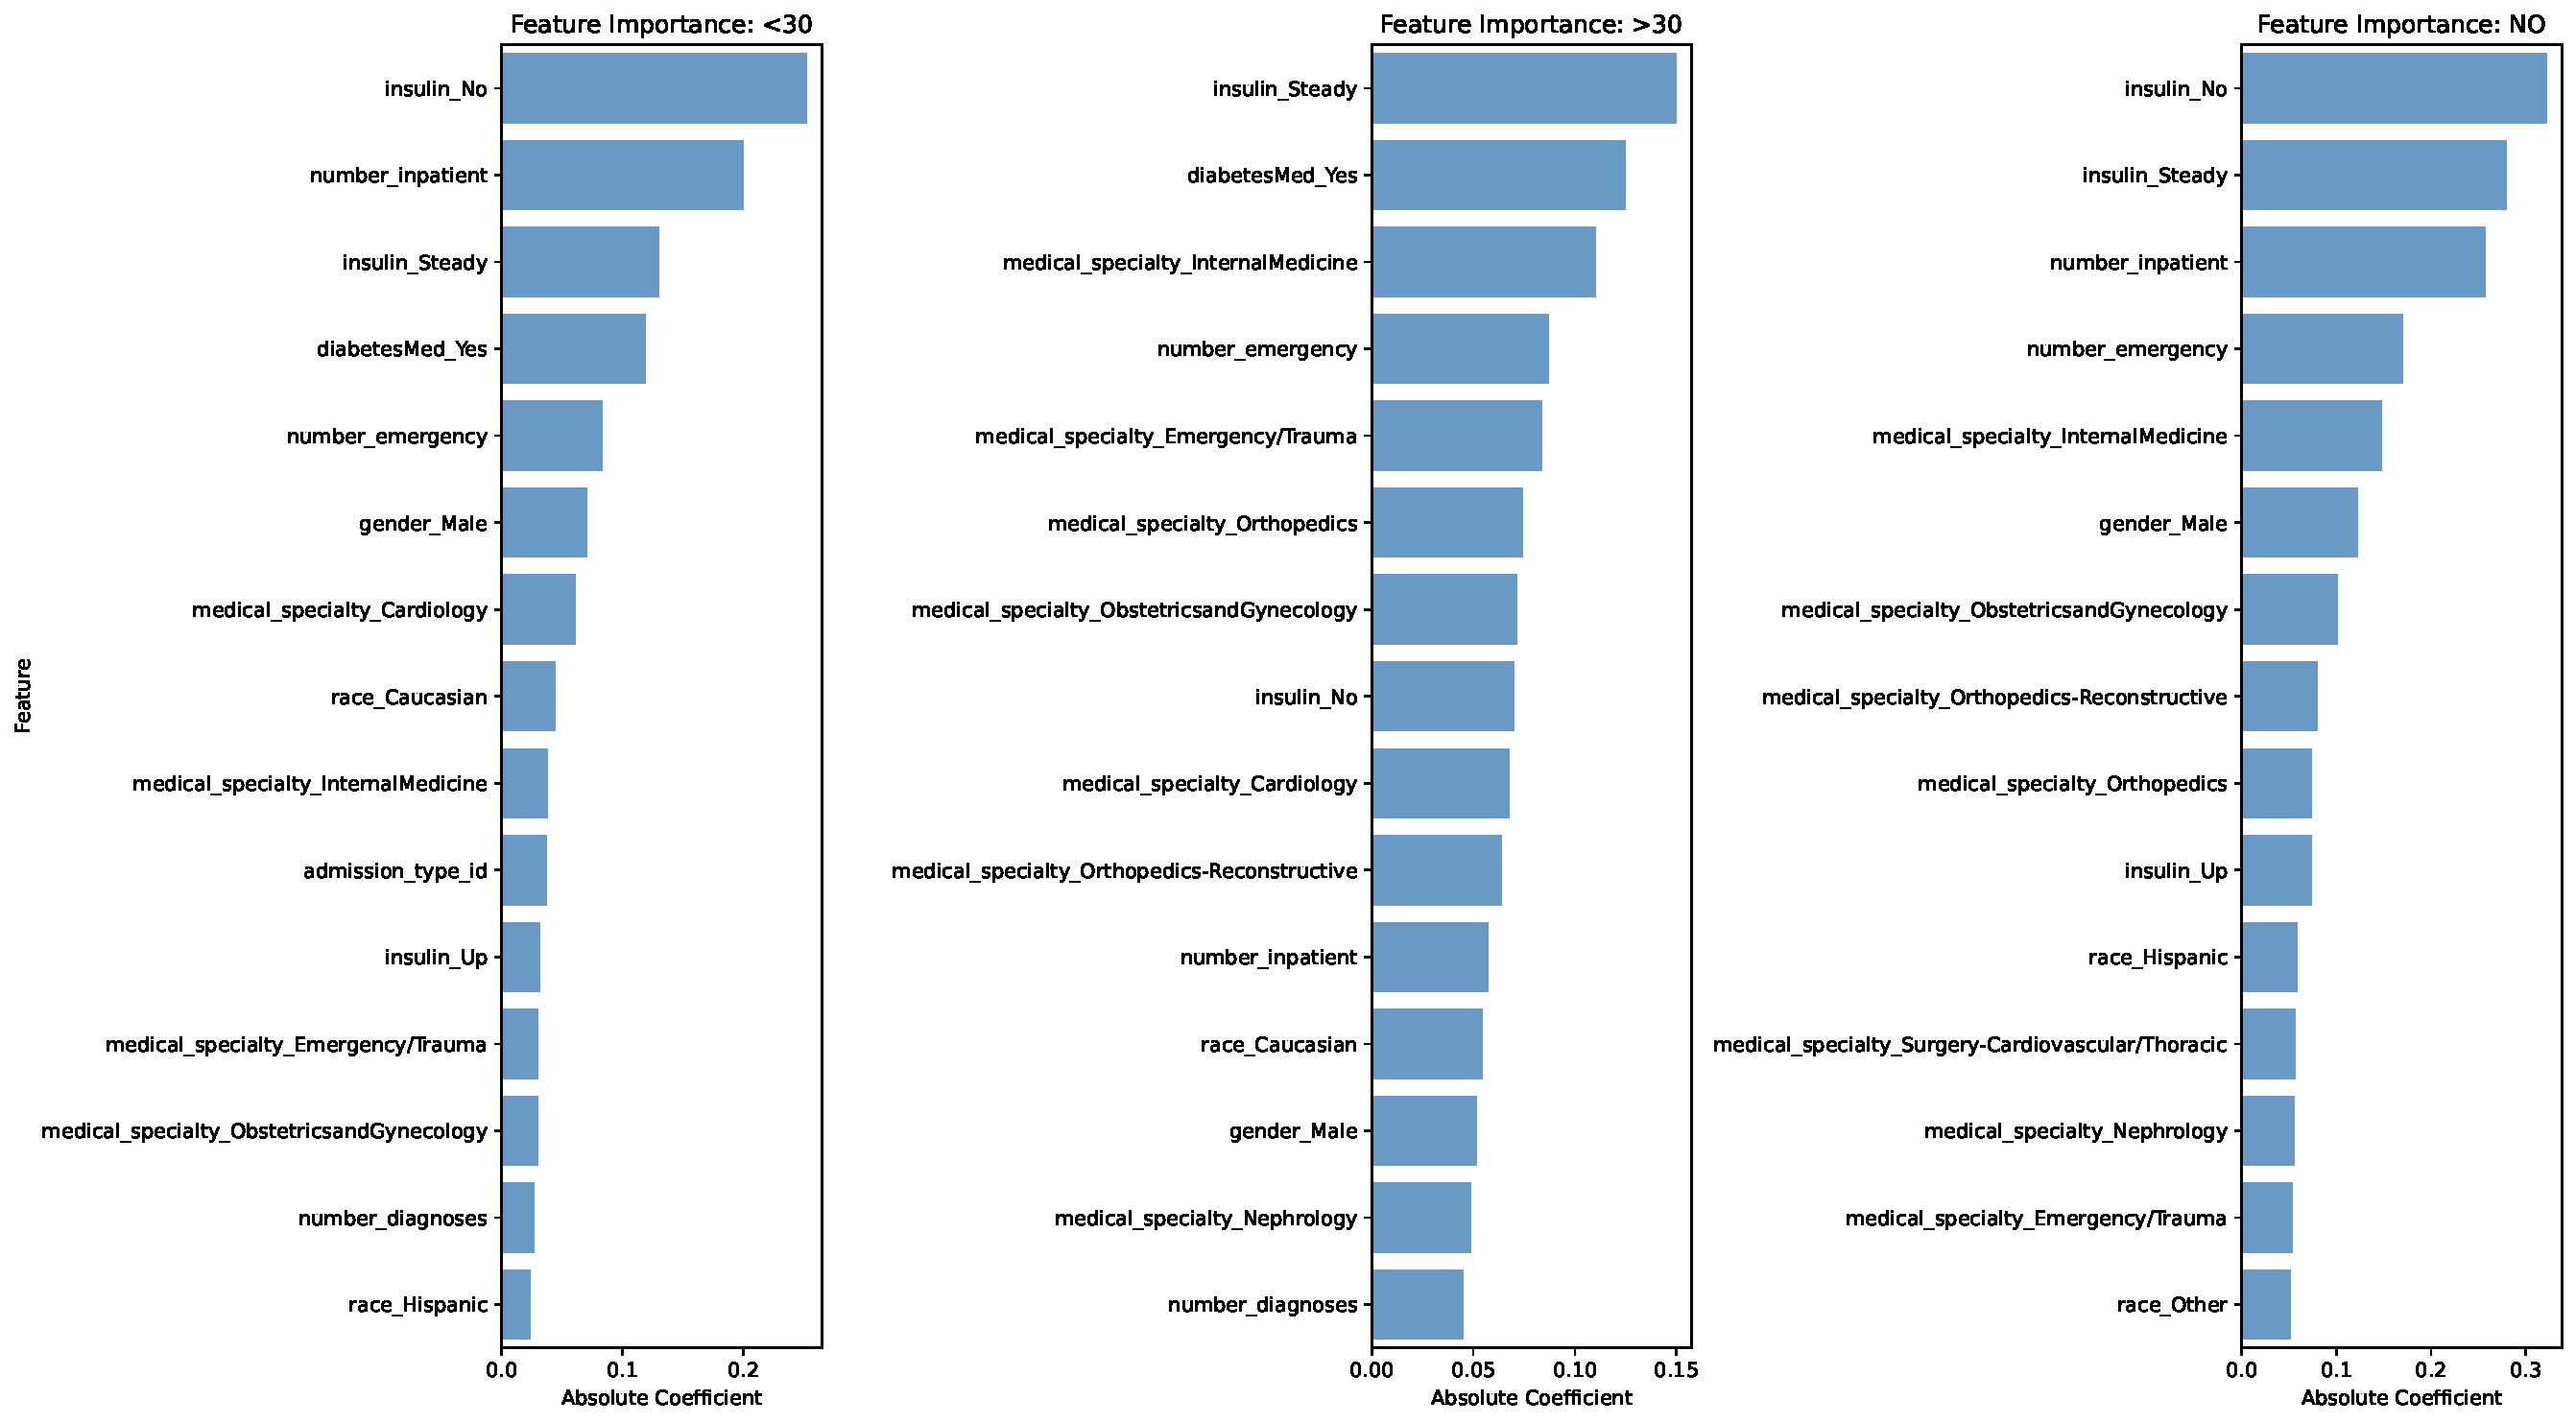
\includegraphics[width=0.9\textwidth]{../figures/feature_importance.pdf}
    \caption{Top 15 features by importance for each readmission category}
    \label{fig:feature_importance}
\end{figure}

\subsection{Key Predictors of Readmission}

Analysis of the feature importance reveals several significant predictors of hospital readmission:

\subsubsection{Readmission within 30 days ("<30")}
\begin{itemize}
    \item Discharge disposition (particularly to skilled nursing facilities)
    \item Number of inpatient visits
    \item Number of diagnoses
    \item Insulin regimen changes
    \item Emergency admission source
\end{itemize}

\subsubsection{Readmission after 30 days (">30")}
\begin{itemize}
    \item Number of medications
    \item Age (older patients)
    \item Longer hospital stays
    \item Specific diagnoses (circulatory system disorders)
    \item Diabetes medication regimen
\end{itemize}

\subsubsection{No Readmission ("NO")}
\begin{itemize}
    \item Discharge to home
    \item Fewer previous inpatient visits
    \item Fewer diagnoses
    \item Non-emergency admissions
    \item Stable medication regimen (no changes during hospitalization)
\end{itemize}

These findings align with clinical intuition and existing literature on hospital readmissions among diabetic patients, reinforcing the validity of the model and providing actionable insights for intervention strategies. 